\documentclass[12pt,a4paper]{article}

\usepackage[utf8]{inputenc}
\usepackage[T1]{fontenc}
\usepackage{lmodern}
\usepackage{amsmath,amssymb,mathtools,bm}
\usepackage{graphicx}
\usepackage{booktabs}
\usepackage{xcolor}
\usepackage[a4paper,margin=20mm]{geometry}
\usepackage[font=small,labelfont=bf,skip=4pt]{caption}
\usepackage[numbers,sort&compress]{natbib}
\usepackage[colorlinks=true,linkcolor=blue!50!black,citecolor=blue!50!black,urlcolor=blue!50!black]{hyperref}

\graphicspath{{figures/}{./}}
\allowdisplaybreaks
\setlength{\textfloatsep}{10pt}
\setlength{\intextsep}{10pt}

\newcommand{\bk}{\mathbf{k}}
\newcommand{\bq}{\mathbf{q}}
\newcommand{\chie}{\chi_{e}}
\newcommand{\chig}{\chi_{\rm geom}}
\newcommand{\chim}{\chi_{\rm mass}}
\newcommand{\Evhs}{E_{\rm vhs}}
\newcommand{\meV}{\,\mathrm{meV}}
\newcommand{\nm}{\,\mathrm{nm}}

\begin{document}

%======================================================================
% Cover page
%======================================================================
\begin{titlepage}
\centering
\vspace*{1cm}
{\Large\bfseries Quantum Geometric Effects at the Monkey Saddle Lifshitz Point\\[4pt] in Biased Bernal Bilayer Graphene\par}
\vspace{1.5cm}
{\itshape Submitted by\par}
\vspace{4pt}
{\large\bfseries Rajat Shuvra Saha\par}
\vspace{4pt}
Integrated M.Sc., 5th year\\
School of Physical Sciences\\
National Institute of Science Education and Research (NISER), Bhubaneswar\\
An OCC of Homi Bhabha National Institute
\vspace{1.5cm}


\includegraphics[width=0.2\textwidth]{niser logo}

\vspace{1.5cm}
{\itshape Under the guidance of\par}
\vspace{4pt}
{\large\bfseries Dr.\ Kush Saha\par}
\vspace{4pt}
Reader-F, School of Physical Sciences\\
National Institute of Science Education and Research (NISER), Bhubaneswar
\vfill
Master's thesis report, November 2026
\end{titlepage}

\pagenumbering{roman}

%======================================================================
% Acknowledgements
%======================================================================
\section*{Acknowledgements}

I would like to thank Dr Kush Saha for his immense contribution to giving the ideas behind the project based on Kitamura's work. I would also like to thank Akash Dey, a Research Associate (RA) currently at NISER, for his contributions to troubleshooting the numerical issues and showing the standard results. Lastly, I would like to thank my parents and close friends for their enduring support to provide encouragement for this project.

\vspace{1cm}
\begin{flushright}
Rajat Shuvra Saha\\
Integrated M.Sc., 5th year\\
School of Physical Sciences\\
NISER Bhubaneswar
\end{flushright}

\clearpage

%======================================================================
% Abstract
%======================================================================
\section*{Abstract}

In Bernal bilayer graphene an interlayer bias tunes the lowest conduction band through a Lifshitz point: at $V_c\simeq40\meV$ its three van Hove saddles merge into a single monkey saddle, a higher-order van Hove singularity whose density of states diverges as a power law. We ask whether the quantum geometry of this band, and not only its dispersion, favours ferromagnetism, as Kitamura, Daido and Yanase recently proposed for singular saddle points. Working with the four-band continuum model, we first obtain the quantum geometric tensor of the critical band in closed form at the saddle. The two interband channels whose cancellation produces the diverging effective mass add in the quantum metric but cancel in the Berry curvature, so the monkey saddle is strongly but almost purely metric-geometric. We then compute the generalized electric susceptibility (GES) $\chie$, the $q^2$ curvature of the bare spin susceptibility, and separate it into a geometric part $\chig$ and an effective-mass part $\chim$. A direct finite-$q$ evaluation of the bubble confirms the separation to better than $1\%$. Near the van Hove energy the sign of $\chie$ is set by the dispersion. Geometry-driven ferromagnetic fluctuations, $\chie<0<\chim$, appear in two well-defined regimes: on the high-density side, $\mu-V/2\gtrsim4.2\meV$, at every bias studied, and at the van Hove energy at low temperature for $V>V_c$. In both regimes $q=0$ is a local, not a global, maximum of $\chi^0(\bq)$. Quantum geometry therefore shapes the magnetic response of the monkey saddle, but as a correction to a dispersion-dominated background and not as its controlling mechanism. A calculation that includes both valleys and goes beyond the random-phase approximation is the natural next step.

\clearpage
\pagenumbering{arabic}

\section{Introduction}\label{sec:intro}
%======================================================================

Van Hove singularities promote electronic instabilities~\citep{VanHove1953}. At an ordinary saddle of a two-dimensional band the density of states diverges logarithmically, and the Stoner criterion $U\nu(E_F)>1$ is met at a smaller interaction strength~\citep{Stoner1938}. When ordinary saddles are brought together by tuning a parameter, the divergence becomes a power law. Such higher-order van Hove singularities~\citep{Shtyk2017,Yuan2019} amplify correlation effects far more strongly, and the point where they appear is called a multicritical Lifshitz point.

Biased Bernal bilayer graphene is a platform to see this in action. Trigonal warping gives the lowest conduction band three saddles near each valley, and the interlayer bias $V$ moves them. At $V_c$ they coalesce into a $C_3$-symmetric cubic monkey saddle~\citep{Shtyk2017}, and the same tunability hosts isospin-polarised metals and spin-polarised superconductivity~\citep{Zhou2022,Seiler2022,delaBarrera2022}. As such, we question the origin of the ferromagnetic response here.

The Stoner argument takes only the dispersion into account. A Bloch state also carries a wavefunction, whose geometry is described by the quantum geometric tensor $Q_n^{\mu\nu}=g_n^{\mu\nu}-\tfrac{i}{2}\Omega_n^{\mu\nu}$. The Berry curvature $\Omega_n$ is only half of it; the quantum metric $g_n$ measures the distance between neighbouring states. Kitamura, Daido and Yanase showed that this distance enters the bare spin susceptibility $\chi^0(\bq)$ through the overlaps of Bloch states~\citep{Kitamura2024}. Its curvature at $q=0$, the generalized electric susceptibility (GES), splits as $\chie=\chig+\chim$: a mass part fixed by the band curvature, and a geometric part whose Fermi-surface metric term always favours ferromagnetism. If $\chie<0$, $q=0$ is a maximum and the ferromagnetic channel leads; otherwise a finite-$q$ channel is preferred. At a singular saddle with a band touching, $g$ diverges and geometry alone makes the ferromagnetic channel win, in the same way that the metric keeps flat-band superconductors superconducting~\citep{Peotta2015,Torma2022}.

The monkey saddle is unexplored territory for this idea. The band is gapped and $g$ stays finite, so it is not obvious whether geometry controls the magnetic response, merely corrects it, or is irrelevant. We ask how large $\chig$ is compared with $\chim$, and whether there are regimes where ferromagnetic fluctuations exist only because of geometry.

We find the following. (i) At the saddle the quantum geometric tensor has a closed form: the two channels that cancel in the effective mass add in $g$ and cancel in $\Omega$. (ii) The density of states is $\nu\propto|E-E_c|^{-1/3}$ with an exact prefactor, and the resulting $T^{-1/3}$ law matches numerics to within $1\%$. (iii) The split $\chie=\chig+\chim$ is verified by a direct finite-$q$ bubble. (iv) Near the van Hove energy the dispersion decides the sign of $\chie$; geometry-driven fluctuations appear at high density, and at the van Hove energy only above $V_c$ at low temperature. (v) There, $q=0$ is only a local maximum of $\chi^0(\bq)$.

Section~\ref{sec:methods} introduces the model and methods, Sec.~\ref{sec:results} presents the results, Sec.~\ref{sec:discussion} discusses them, and Sec.~\ref{sec:conclusions} concludes.
%======================================================================
\section{Model and methods}\label{sec:methods}
%======================================================================

\subsection{Four-band model and the critical bias}\label{sec:model}

We use the four-band continuum Hamiltonian of Bernal bilayer graphene near valley $K$~\citep{McCann2006,McCann2013}, in the basis $(A_1,B_1,A_2,B_2)$,
\begin{equation}
H(\bk)=\begin{pmatrix}
V/2 & v\pi^\dagger & 0 & v_3\pi\\
v\pi & V/2 & \gamma_1 & 0\\
0 & \gamma_1 & -V/2 & v\pi^\dagger\\
v_3\pi^\dagger & 0 & v\pi & -V/2
\end{pmatrix},\qquad \pi=k_x+ik_y,
\label{eq:H}
\end{equation}
where $v=0.658\,$eV\,nm is the intralayer velocity, $\gamma_1=0.40\,$eV couples the dimer sites $B_1$ and $A_2$, $v_3=0.1\,v$ describes trigonal warping, and $V$ is the interlayer bias. We study the lowest conduction band, band~3 counted from below. At $\bk=0$ it is the pure $A_1$ orbital at energy $V/2$. A useful feature of Eq.~\eqref{eq:H} is that it is linear in $\bk$: the velocity matrices $\partial_{k_i}H$ are constant, so every band derivative needed below is an exact finite sum over the four states. We exploit this both analytically and numerically.

Eliminating the dimer orbitals $(B_1,A_2)$ gives, to leading order (Appendix~\ref{app:dispersion}),
\begin{equation}
\varepsilon_3(\bk)-\frac V2\simeq \alpha(V)\,k^2-A\,k^3\cos3\varphi+B\,k^4,\qquad
\alpha(V)=\frac{v_3^2}{V}-\frac{v^2V}{\gamma_1^2}.
\label{eq:disp}
\end{equation}
The coefficient $\alpha$ has a simple meaning. Direct hopping from $A_1$ to $B_2$, of strength $v_3$, pushes the band up; virtual hopping through the dimer pushes it down. The two compete, and they cancel exactly at
\begin{equation}
V_c=\frac{\gamma_1v_3}{v}=40\meV .
\end{equation}
At this bias the band has no quadratic term at all. Its shape is fixed by the cubic coefficient $A=2v^3/\gamma_1^2$, and the quartic coefficient $B=v^5/(\gamma_1^3v_3)$ takes over beyond the crossover scales
\begin{equation}
k_*=A/B=0.122\nm^{-1},\qquad E_*=A^4/B^3=6.40\meV .
\end{equation}
These set the natural units of the problem. Throughout we measure the bias by $\delta\equiv V/V_c$.

\subsection{Quantum geometric tensor}\label{sec:qgt}

The quantum geometric tensor of band $n$,
$Q^n_{\mu\nu}=\langle\partial_\mu u_n|(1-|u_n\rangle\langle u_n|)|\partial_\nu u_n\rangle=g^n_{\mu\nu}-\tfrac i2\Omega^n_{\mu\nu}$,
contains the quantum metric $g$, which measures the distance between neighbouring Bloch states, and the Berry curvature $\Omega$~\citep{Provost1980}. For a Hamiltonian linear in $\bk$ both follow from the interband velocity matrix elements $v^\mu_{nm}=\langle n|\partial_\mu H|m\rangle$:
\begin{equation}
g^n_{\mu\nu}=\sum_{m\neq n}\frac{\mathrm{Re}\,v^\mu_{nm}v^\nu_{mn}}{(\varepsilon_n-\varepsilon_m)^2},\qquad
\Omega^n_{xy}=-2\sum_{m\neq n}\frac{\mathrm{Im}\,v^x_{nm}v^y_{mn}}{(\varepsilon_n-\varepsilon_m)^2}.
\label{eq:qgt}
\end{equation}

\subsection{Generalized electric susceptibility}\label{sec:ges}

The bare spin susceptibility, per spin and per valley, is
\begin{equation}
\chi^0(\bq)=-\sum_{nm}\int\!\frac{d^2k}{(2\pi)^2}\,
\frac{f(\varepsilon_{n,\bk_-})-f(\varepsilon_{m,\bk_+})}{\varepsilon_{n,\bk_-}-\varepsilon_{m,\bk_+}}
\,\big|\langle u_{n,\bk_-}|u_{m,\bk_+}\rangle\big|^2,\qquad \bk_\pm=\bk\pm\bq/2 ,
\label{eq:bubble}
\end{equation}
where $f$ is the Fermi function. The wavefunctions enter only through the overlaps, and it is through them that quantum geometry affects the response. Following Ref.~\citep{Kitamura2024}, the GES is the curvature of $\chi^0$ at the origin,
\begin{equation}
\chie\equiv\lim_{\bq\to0}\partial_{q_x}^2\chi^0(\bq),\qquad
\chi^0(\bq)\simeq\chi^0(0)\big(1-\ell^2q^2\big),\qquad \ell^2=-\frac{\chie}{2\chi^0(0)} .
\label{eq:GESdef}
\end{equation}
$C_3$ symmetry makes the curvature tensor isotropic, so one number suffices. Its sign has a direct physical meaning. If $\chie<0$, then $q=0$ is a maximum of $\chi^0$. Within the random-phase approximation, $\chi_s=\chi^0_s/(1-U\chi^0_s)$, the Stoner instability is then reached first in the uniform channel, and the paramagnetic state has ferromagnetic fluctuations. The length $\ell$ measures how sharp the peak is.

Expanding Eq.~\eqref{eq:bubble} to order $q^2$ (Appendix~\ref{app:ges}) gives $\chie=\chig+\chim$, with
\begin{align}
\chig&=2\sum_n\int\!\frac{d^2k}{(2\pi)^2}\Big[\frac{f'(\varepsilon_n)}{2}\,g^{n}_{K}+f(\varepsilon_n)\,X_n\Big], \label{eq:chig}\\
\chim&=-2\sum_n\int\!\frac{d^2k}{(2\pi)^2}\,\frac{f''(\varepsilon_n)}{12}\,\big[m_n^{-1}\big], \label{eq:chim}
\end{align}
which is the form given by Kitamura \emph{et al.} Here $g_K$ is twice the direction-averaged metric of Eq.~\eqref{eq:qgt}, $X_n$ is an interband (positional-shift) term, and $[m_n^{-1}]$ is the inverse effective mass; explicit expressions are given in Appendix~\ref{app:ges}. The mass term is all that would remain if the Bloch states did not depend on $\bk$.

Two properties of these formulas organise all the results that follow. First, the Fermi-surface metric term is always negative, because $f'\le0$. At the Fermi surface, geometry always pushes towards ferromagnetism, although the Fermi-sea term $X_n$ can partly compensate it. Second, $f''(\varepsilon-\mu)$ is odd about $\mu$. Hence $\chim$ measures the \emph{imbalance} of band curvature between states just below and just above $\mu$. Near a saddle both sides are large and of opposite curvature, so $\chim$ is large and changes sign as $\mu$ crosses $\Evhs$. These two properties suggest a sharp criterion. We call a ferromagnetic fluctuation \emph{geometry driven} when $\chie<0$ but $\chim>0$, that is, when the dispersion alone would make $q=0$ a minimum of $\chi^0$ and only the wavefunctions turn it into a maximum.

\subsection{Numerical method}\label{sec:numerics}

Critical points of $\varepsilon_3$ are located on the mirror lines of the band and classified by its exact Hessian. All momentum integrals are evaluated on Gauss--Legendre polar grids, with full Fermi functions for all four bands. Numerical details and convergence tests are given in Appendix~\ref{app:numerics}. Results are quoted per spin and per valley; the $K'$ valley contributes identically by time-reversal symmetry.

%======================================================================
\section{Results}\label{sec:results}
%======================================================================

\subsection{The monkey saddle and the three saddle phases}\label{sec:phases}

For $\delta\neq1$ and small $|\alpha|$, Eq.~\eqref{eq:disp} has three ordinary saddles at $|\bk_s|=2|\alpha|/3A$, with energy
\begin{equation}
\Evhs-\frac V2\simeq\frac{4\alpha^3}{27A^2}.
\label{eq:Evhs}
\end{equation}
Figure~\ref{fig:phases} shows the resulting three saddle phases, and Table~\ref{tab:crit} in Appendix~\ref{app:numerics} lists their critical points. For $\delta<1$, $\bk=0$ is a local minimum surrounded by three saddles on the rays $\varphi=0,\pm2\pi/3$. At $\delta=1$ the three saddles have merged into the monkey saddle (Fig.~\ref{fig:monkey}). For $\delta>1$, $\bk=0$ is a local maximum and the saddles reappear rotated by $\pi/3$. In all three phases the band bottom lies in three minivalleys at $|\bk|\approx0.6$--$0.9\,k_*$. At $\delta=1$ the density of states diverges as
$\nu(E)\simeq0.0615\,A^{-2/3}|E-E_c|^{-1/3}$, which we derive with its prefactor in Appendix~\ref{app:dispersion}. This power law is the property that makes the monkey saddle attractive for instabilities.

\begin{figure}[t]
\centering
\begin{minipage}[c]{0.36\textwidth}\centering
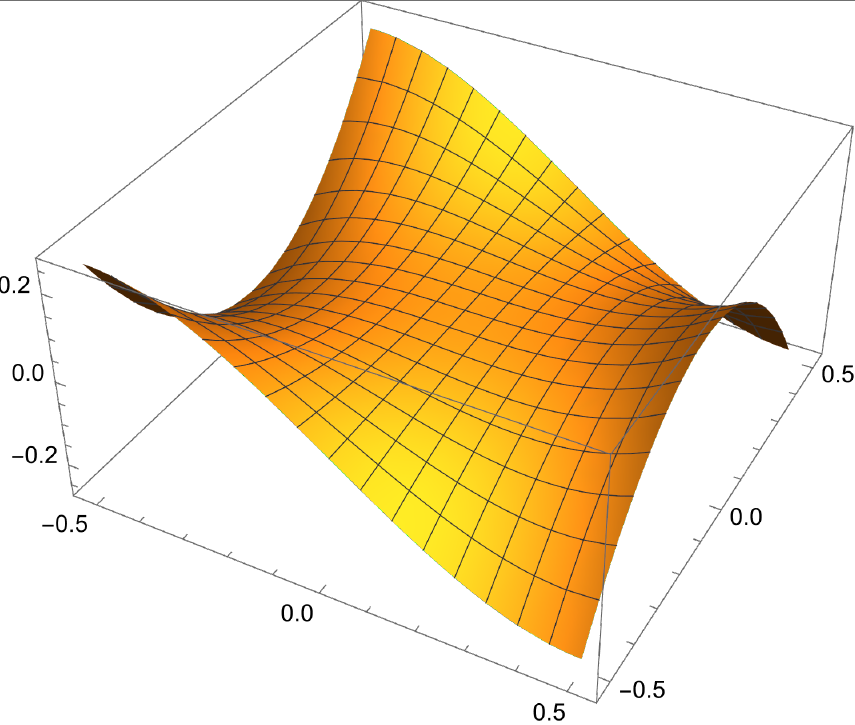
\includegraphics[width=\textwidth]{Monkey_Saddle_3D_Plot.png}
\end{minipage}\hfill
\begin{minipage}[c]{0.60\textwidth}
\caption{The monkey saddle. Dispersion $\varepsilon_3(\bk)-V_c/2$ of the critical band at $V=V_c$ near $\bk=0$. The surface rises along three directions and falls along the three in between, the cubic shape $-Ak^3\cos3\varphi$ of Eq.~\eqref{eq:disp}. The Hessian vanishes at the centre, so the density of states diverges as $|E-E_c|^{-1/3}$ rather than logarithmically.}
\label{fig:monkey}
\end{minipage}
\end{figure}

\begin{figure}[t]
\centering
\begin{minipage}[t]{0.60\textwidth}\centering
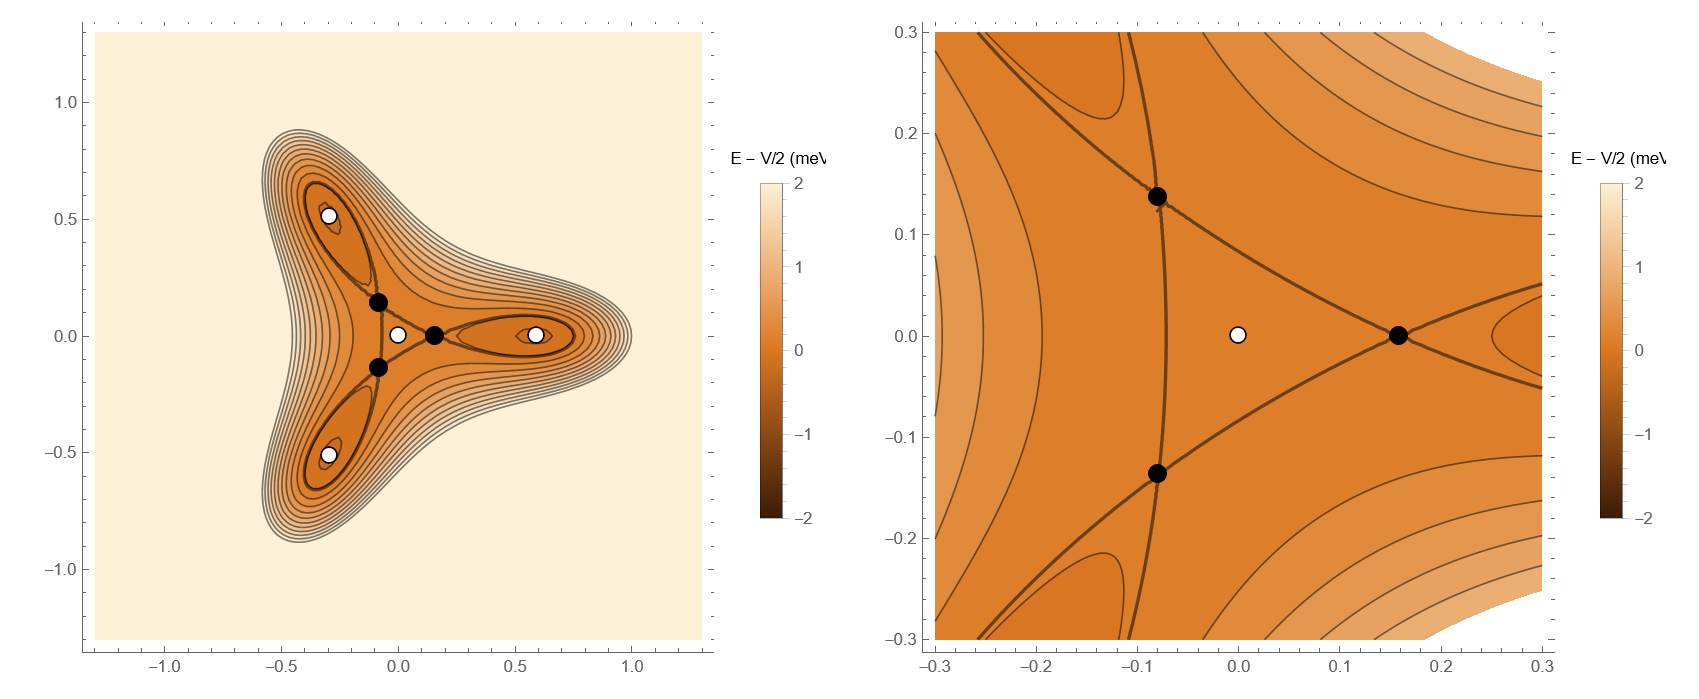
\includegraphics[width=\textwidth]{Undergapped_state.png}\\[-2pt]
{\small (a)}
\end{minipage}\\[4pt]
\begin{minipage}[t]{0.495\textwidth}\centering
\includegraphics[width=\textwidth]{{Delta=1.0}.png}\\[-2pt]
{\small (b)}
\end{minipage}\hfill
\begin{minipage}[t]{0.495\textwidth}\centering
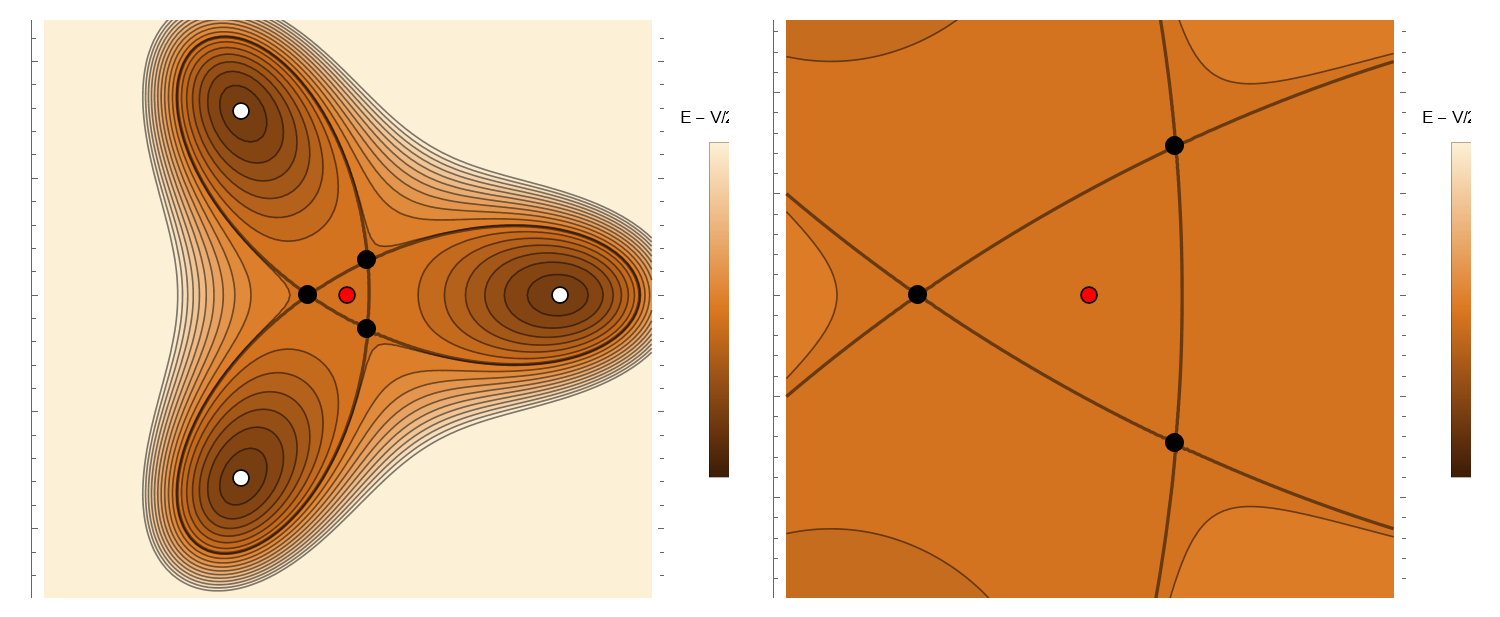
\includegraphics[width=\textwidth]{Overgapped.png}\\[-2pt]
{\small (c)}
\end{minipage}
\caption{The three saddle phases of the critical band. (a) $\delta=0.5$: minimum at $\bk=0$ (white) and three saddles (black). (b) $\delta=1.0$: monkey saddle (red). (c) $\delta=1.5$: maximum at $\bk=0$ (red), saddles rotated by $\pi/3$. Colour: $\varepsilon_3-V/2$ in meV, clipped at $\pm2\meV$. Axes: $k_{x,y}/k_*$. In each pair the right panel is a zoom to $|k|\le0.3\,k_*$. The thick contour is the van Hove energy, and white circles mark the minivalley minima.}
\label{fig:phases}
\end{figure}

\subsection{Quantum geometry of the critical band}\label{sec:geometry}

At $\bk=0$ only two channels contribute to Eq.~\eqref{eq:qgt}, and they are the same two that compete in $\alpha(V)$. Appendix~\ref{app:geometry} shows that
\begin{equation}
g_{xx}=g_{yy}=\underbrace{\frac{v_3^2}{V^2}}_{B_2}+\underbrace{\frac{v^2(\gamma_1^2+V^2)}{\gamma_1^4}}_{\rm dimer},\qquad g_{xy}=0,\qquad
\Omega_{xy}=\frac{2v_3^2}{V^2}-\frac{2v^2(\gamma_1^2+V^2)}{\gamma_1^4}.
\label{eq:gOmega}
\end{equation}
The relative sign between the two expressions is the central observation of this section. The $B_2$ channel couples to band 3 through $\pi$ and the dimer channel through $\pi^\dagger$, so the two carry opposite chirality. Each saturates the bound $|\Omega|\le2\sqrt{\det g}$ on its own. Their metrics, being positive, add; their Berry curvatures, having opposite signs, cancel.

Near $V_c$ the two channels are almost equal in magnitude. This is the same balance that makes $\alpha(V_c)=0$, up to a correction of order $V^2/\gamma_1^2$. The Lifshitz point is therefore also a point of almost perfect Berry-curvature cancellation (Table~\ref{tab:geo}). At $V_c$ the metric is $g=5.44\nm^2$, half of it from the remote dimer bands, while $\Omega$ passes through zero at $V=0.995\,V_c$. Away from $\bk=0$, the metric and the curvature are concentrated in three lobes near $|\bk|\approx k_*$, beyond the tips of the van Hove contour. We conclude that the geometry relevant to the monkey saddle is \emph{metric dominated}. This matters because the quantum metric, and not the Berry curvature, is what enters the GES.

\begin{table}[t]
\centering
\caption{Effective-mass coefficient and quantum geometry of band 3 at $\bk=0$, Eqs.~\eqref{eq:disp} and \eqref{eq:gOmega}. Exact diagonalisation agrees to all digits shown.}
\label{tab:geo}
\small
\begin{tabular}{ccccc}
\toprule
$\delta$ & $\alpha$ (eV\,nm$^2$) & $g_{xx}(\bk=0)$ (nm$^2$) & $\Omega_{xy}(\bk=0)$ (nm$^2$) & dimer share of $g$\\
\midrule
0.5 & $+0.162$ & 13.54 & $+16.22$ & 0.20\\
1.0 & $0$ & 5.44 & $-0.05$ & 0.50\\
1.5 & $-0.090$ & 3.97 & $-3.13$ & 0.69\\
\bottomrule
\end{tabular}
\end{table}

\subsection{Dependence on chemical potential}\label{sec:mu}

Figure~\ref{fig:gesmu} shows the three components of the GES against chemical potential at $T=0.1\meV$, for $\delta=0.8$, $1$ and $1.2$.

\emph{Near the van Hove energy} (top row) both components are tens of eV$^{-1}$. As anticipated, $\chim$ changes sign at $\Evhs$, and it controls the sign of $\chie$. Just below $\Evhs$ there is a ferromagnetic window, but it is mostly dispersion driven (grey). Geometry only widens it, adding the narrow orange strip at its upper edge.

\emph{On the high-density side} (bottom row) the picture is different. Both components are an order of magnitude smaller, and $\chim$ stays positive. But $\chig$ is negative and larger in magnitude, so from $\mu-V/2\approx4.2\meV$ upward $\chie<0$ purely because of geometry. This window is essentially independent of bias. At $\mu-V/2=8\meV$ and $V=V_c$ we find $\chie=-0.30$ and $\chim=+1.57\,$eV$^{-1}$: geometry turns a dip of the bubble at $q=0$ ($\ell^2=-6.8\nm^2$) into a peak ($\ell^2=+1.3\nm^2$).

\begin{figure}[t]
\centering
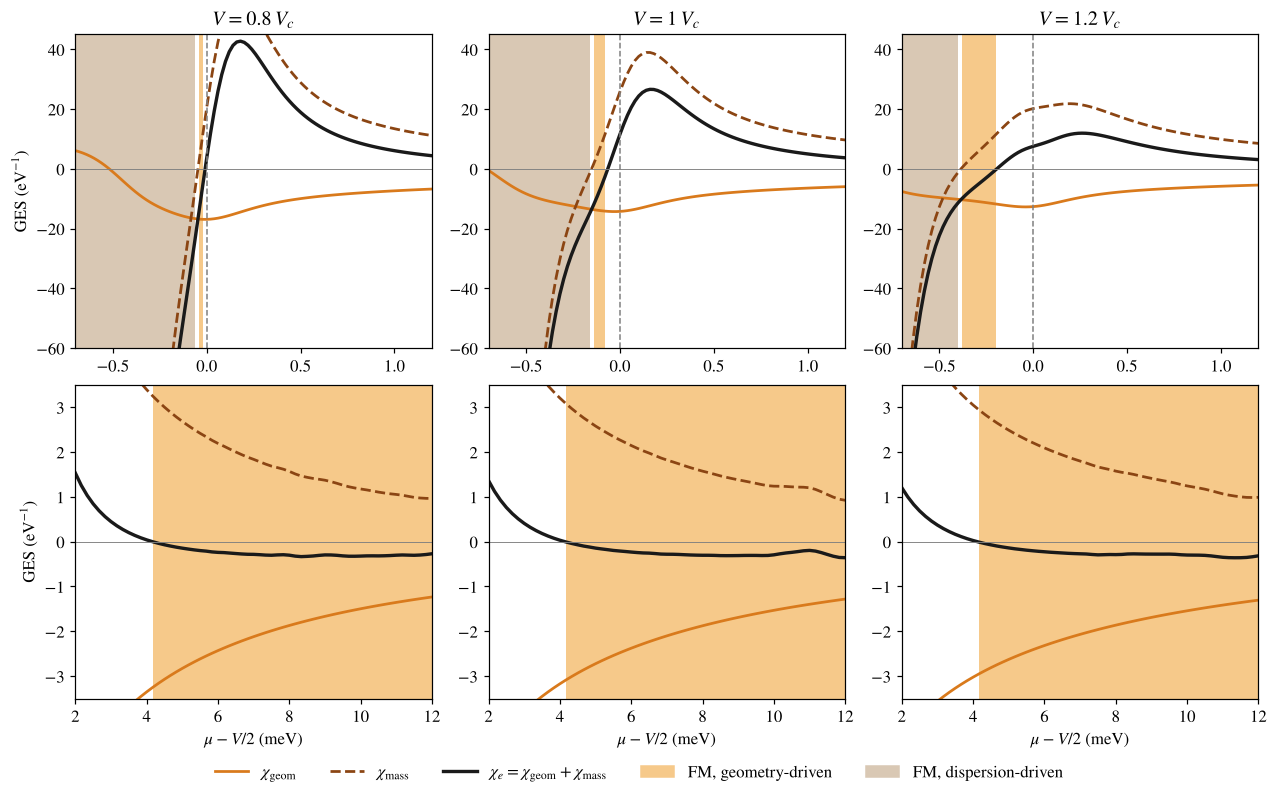
\includegraphics[width=0.74\textwidth]{GES_ipynb_Biased.png}
\caption{GES components against chemical potential at $T=0.1\meV$. Top: near the van Hove energy (dashed vertical line). Bottom: high-density side. Orange shading: geometry-driven ferromagnetic fluctuation ($\chie<0<\chim$). Grey: dispersion-driven ($\chie<0$, $\chim<0$).}
\label{fig:gesmu}
\end{figure}

\subsection{Temperature dependence at the van Hove energy}\label{sec:T}

Figure~\ref{fig:Tsweep} follows the three components at $\mu=\Evhs$ from $1.16$ to $116\,$K ($0.1$--$10\meV$) in the three saddle phases. Over this range the thermal window reaches the valence band, which lies only $V$ below, so all four bands are treated with full Fermi functions.

The three phases behave in qualitatively different ways. At $\delta=0.5$, $\chim$ is large and negative at all temperatures, with a minimum of $-65\,$eV$^{-1}$ near $2\,$K, and $\chie$ reaches $-83\,$eV$^{-1}$. The ferromagnetic tendency is strong but entirely dispersion driven.

At $\delta=1$ and the lowest temperature, $\chim=+26\,$eV$^{-1}$ outweighs $\chig=-14\,$eV$^{-1}$, so $\chie>0$: at the lowest temperature studied, the system tuned exactly to the monkey saddle does \emph{not} favour $q=0$. $\chim$ changes sign near $2.5\,$K, and $\chie$ is negative between $1.8$ and $79\,$K. Geometry decides the sign only in the narrow interval $1.9$--$2.5\,$K.

At $\delta=1.5$, $\chie$ is negative over the whole range, and below $5\,$K $\chim>0$ while $\chie<0$. At the van Hove energy above $V_c$, the low-temperature ferromagnetic tendency is therefore \emph{geometry driven}.

In all three cases $\chig$ is most negative at low temperature and turns positive at high temperature, at $16$, $34$ and $63\,$K respectively. The reason is thermal occupation of the valence band, which makes the positive Fermi-sea term dominate. The geometric advantage is thus a low-temperature effect.

\begin{figure}[t]
\centering
\begin{minipage}[t]{0.325\textwidth}\centering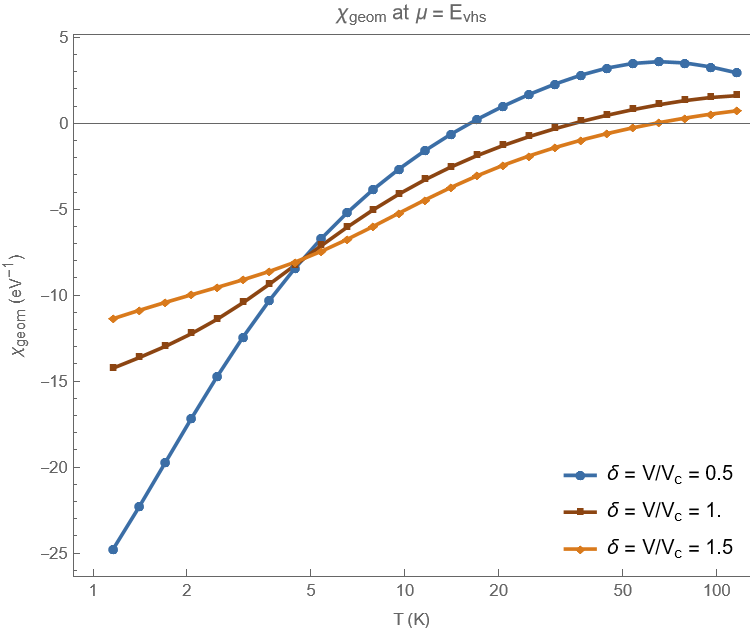
\includegraphics[width=\textwidth]{chi_geom_Temperature_Scan_Biased.png}\\{\small (a) $\chig$}\end{minipage}\hfill
\begin{minipage}[t]{0.325\textwidth}\centering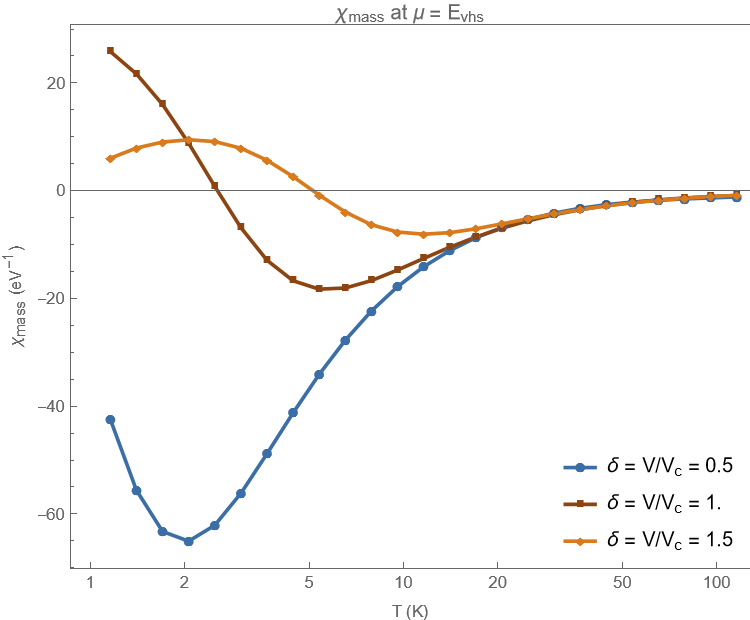
\includegraphics[width=\textwidth]{chi_mass_Temperature_Scan_Biased.png}\\{\small (b) $\chim$}\end{minipage}\hfill
\begin{minipage}[t]{0.325\textwidth}\centering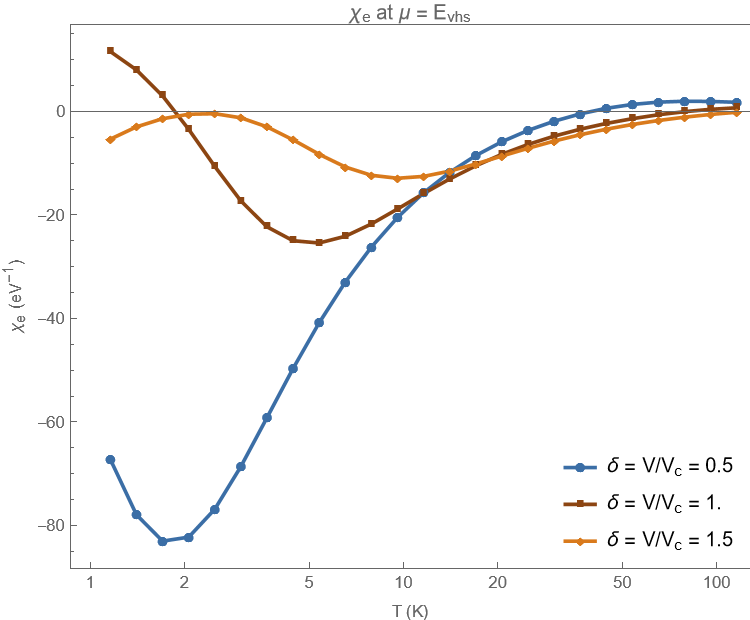
\includegraphics[width=\textwidth]{chi_total_temp_scan_biased.png}\\{\small (c) $\chie=\chig+\chim$}\end{minipage}
\caption{Temperature dependence of the GES at $\mu=\Evhs$ for $\delta=0.5$, $1$ and $1.5$, from $1.16$ to $116\,$K.}
\label{fig:Tsweep}
\end{figure}

The uniform susceptibility places these numbers in context (Appendix~\ref{app:supp}, Fig.~\ref{fig:chi0}). At $\mu=\Evhs$ and $V=V_c$ it follows $\chi^0(0)\propto T^{-1/3}$ below about $0.1\meV$, and its prefactor agrees with the analytic result $\chi^0(0)\simeq0.0702\,A^{-2/3}T^{-1/3}$ of Appendix~\ref{app:dispersion} to better than $1\%$, a stringent test of the numerics. In the high-density window the sign difference between the full and the dispersion-only GES is robust: $\chie\approx-0.3$ against $\chim\approx+1.6\,$eV$^{-1}$ at every temperature and bias shown.

\subsection{Direct test at finite $q$}\label{sec:finiteq}

The GES describes only the curvature of $\chi^0(\bq)$ at the origin. To test both the decomposition and its physical meaning, we evaluate Eq.~\eqref{eq:bubble} directly at finite $q\hat{\mathbf{x}}$, for $V=V_c$, $\mu-V/2=8\meV$ and $T=0.2\meV$. We compare the full four-band model with a geometrically trivial model that has the same band energies but overlaps replaced by $\delta_{nm}$ (Fig.~\ref{fig:finiteq}).

The small-$q$ curvatures are $-0.152$ for the full model and $+0.790$ for the trivial one. The GES formulas predict $\chie/2=-0.151$ and $\chim/2=+0.788$. The agreement confirms Eqs.~\eqref{eq:chig} and~\eqref{eq:chim} by a calculation that shares no intermediate step with them. It also shows the effect in the plainest possible way: with geometry $q=0$ is a maximum, without it a minimum.

The full range of $q$ adds an important qualification. The maximum at $q=0$ is only local. The bubble has its global maximum at $q\approx0.28\nm^{-1}$, about $15\%$ above $\chi^0(0)$. Within the random-phase approximation an instability at this filling would therefore first appear at a finite wavevector.

\begin{figure}[t]
\centering
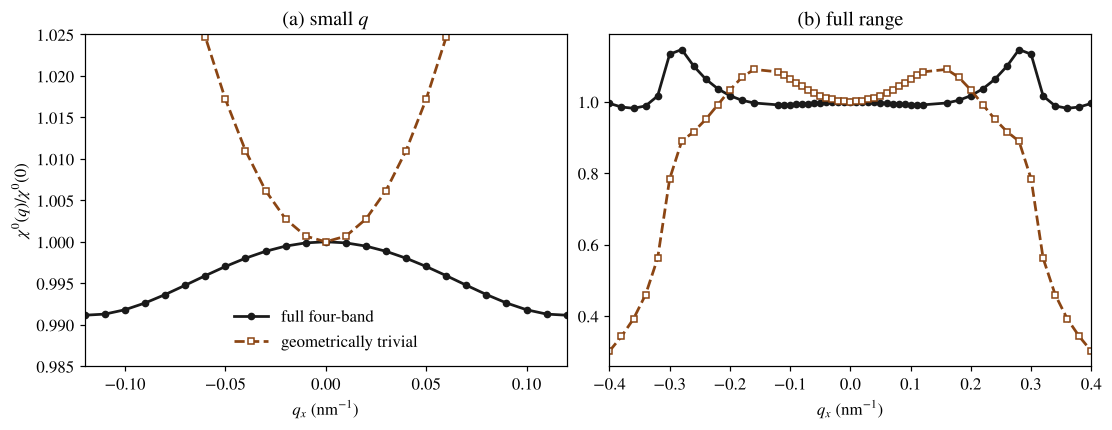
\includegraphics[width=0.80\textwidth]{fullfour_band_comparison_ipynb.png}
\caption{Bare susceptibility at finite $q$ for $V=V_c$, $\mu-V/2=8\meV$ and $T=0.2\meV$. Full four-band model (solid) and geometrically trivial model (dashed). (a) Small $q$: geometry turns the minimum at $q=0$ into a maximum. (b) Full range: the global maximum lies at $q\approx0.28\nm^{-1}$.}
\label{fig:finiteq}
\end{figure}

\subsection{Phase diagram of geometry-driven fluctuations}\label{sec:map}

Figure~\ref{fig:map} summarises the classification at $V=V_c$ in the $(\mu,T)$ plane. Near the monkey saddle the dispersion-driven region dominates. The geometry-driven region is a thin band along its boundary, which moves to higher $\mu$ as $T$ grows. On the high-density side the geometry-driven region is large, and sharply bounded at $\mu-V/2\approx4.2\meV$; this boundary moves only slightly up to $T\approx0.7\meV$.

\begin{figure}[t]
\centering
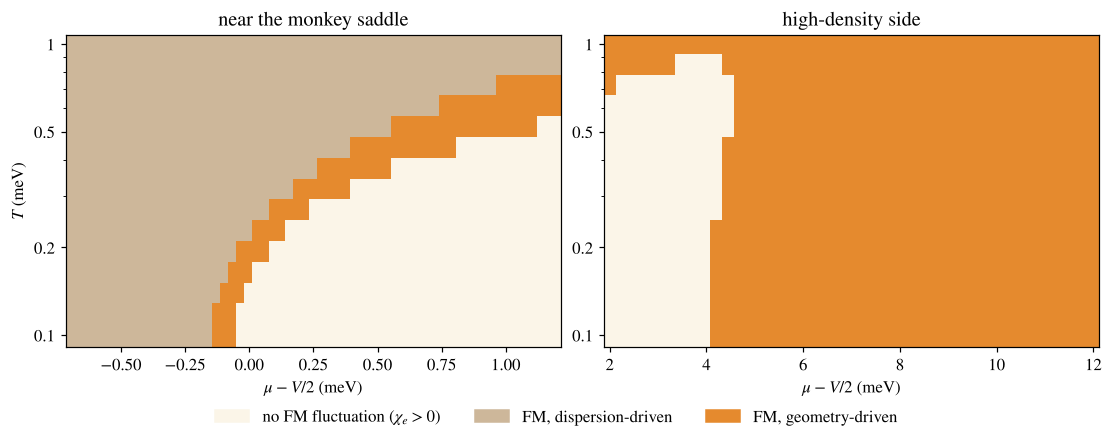
\includegraphics[width=0.80\textwidth]{Monkey_Saddle_Phase_Diagram.png}
\caption{Character of the $q=0$ response at $V=V_c$. Orange: geometry-driven ferromagnetic fluctuation ($\chie<0<\chim$). Brown: dispersion-driven ($\chie<0$, $\chim<0$). Cream: $q=0$ is a minimum of $\chi^0$.}
\label{fig:map}
\end{figure}

%======================================================================
\section{Discussion}\label{sec:discussion}
%======================================================================

\subsection{Physical picture}

The results fit into one picture. The monkey saddle arises because two virtual processes, hopping to $B_2$ and hopping through the dimer, cancel in the band curvature. The same two processes add in the quantum metric and cancel in the Berry curvature. The critical band is therefore strongly, and almost purely, metric-geometric, with $g\simeq5.4\nm^2$ at $\bk=0$ and $\Omega_{xy}\approx0$ (Table~\ref{tab:geo}).

This geometry does enter the spin response, and the decomposition $\chie=\chig+\chim$ quantifies how. Its effect is selective, for a reason that follows from the second property in Sec.~\ref{sec:ges}. A saddle is precisely a place where the band curvature is large and changes sign with energy, so near $\Evhs$ the mass term is large and sets the sign of $\chie$ (Fig.~\ref{fig:gesmu}, top). Geometry can decide the outcome only where the dispersion is nearly neutral. That happens in two places: on the high-density side, where both terms are small and $\chig$ is the larger (Fig.~\ref{fig:gesmu}, bottom), and at the van Hove energy above $V_c$, where the rotated saddles make $\chim$ positive at low temperature (Fig.~\ref{fig:Tsweep}). In both regimes the peak of $\chi^0(\bq)$ at $q=0$ is local, and a finite-$q$ maximum competes with it (Fig.~\ref{fig:finiteq}).

\subsection{Comparison with the singular saddle point}

It is instructive to compare with the singular saddle of Kitamura \emph{et al.}, which we reproduce as a benchmark in Appendix~\ref{app:benchmark}. There the saddle sits at a band touching, the metric diverges, and $\chig$ overwhelms a positive $\chim$ as the gap closes (Fig.~\ref{fig:bench}). The monkey saddle is singular in its dispersion but regular in its geometry: the band is gapped and its metric stays finite. This is why, in bilayer graphene, quantum geometry is a sizeable correction and not the controlling mechanism. The comparison suggests a general lesson. A higher-order van Hove singularity enhances the density of states, but geometry-driven magnetism requires in addition a small interband gap at the saddle.

\subsection{Limitations and outlook}

Several limitations should be kept in mind. First, our conclusions concern the bare bubble. Interactions enter only through the random-phase argument, and vertex corrections may change the balance between $q=0$ and the finite-$q$ maximum of Fig.~\ref{fig:finiteq}. Second, the calculation is for one valley and one spin; intervalley processes, which are relevant to the isospin order seen experimentally~\citep{Zhou2022,Seiler2022,delaBarrera2022}, are not included. Third, the model keeps only $\gamma_1$, $v$ and $v_3$. Further hopping terms, such as the skew interlayer coupling, would shift $V_c$ and change the dispersion quantitatively. We expect, but have not checked, that the opposite chirality of the two channels, on which the metric-dominated geometry rests, survives. Each limitation points to a natural extension: a two-valley calculation of the full isospin susceptibility, an interacting treatment that follows the finite-$q$ maximum into an ordered state, and a quantitative comparison with the gate-tuned phase diagrams of Refs.~\citep{Zhou2022,Seiler2022,delaBarrera2022}.

%======================================================================
\section{Conclusions}\label{sec:conclusions}
%======================================================================

We have studied the interplay of a higher-order van Hove singularity and quantum geometry in biased Bernal bilayer graphene. As the bias crosses $V_c$, three ordinary saddles of the lowest conduction band merge into a monkey saddle and reappear rotated by $\pi/3$ (Figs.~\ref{fig:monkey} and~\ref{fig:phases}); at $V_c$ the density of states diverges as $|E-E_c|^{-1/3}$, with a prefactor we obtain analytically. The band at the saddle carries a large quantum metric and an almost vanishing Berry curvature, because the two interband channels that cancel in the effective mass have opposite chirality.

The generalized electric susceptibility separates cleanly into geometric and effective-mass parts, and a direct finite-$q$ calculation confirms the separation. Near the van Hove energy the dispersion controls the sign of $\chie$. Geometry-driven ferromagnetic fluctuations appear on the high-density side, $\mu-V/2\gtrsim4.2\meV$, at all biases studied, and at the van Hove energy for $T\lesssim5\,$K above $V_c$ (Fig.~\ref{fig:map}). In these regimes the peak of $\chi^0(\bq)$ at $q=0$ is local, and a finite-$q$ maximum competes with it.

The monkey saddle thus realises the mechanism of Kitamura \emph{et al.} in a gapped, experimentally accessible band, but in a weaker form than at a singular saddle point: quantum geometry decides the character of the magnetic response only where the dispersion is nearly neutral.


\bibliographystyle{unsrtnat}
\bibliography{refs.bib}

%======================================================================
\clearpage
\appendix
\section{Effective dispersion and the critical bias}\label{app:dispersion}
%======================================================================

For $|E|,\,vk\ll\gamma_1$ the dimer orbitals $(B_1,A_2)$ can be eliminated. To second order in the couplings this gives the two-band Hamiltonian in the $(A_1,B_2)$ basis~\citep{McCann2013}
\begin{equation}
h(\bk)=\begin{pmatrix}\frac V2\Big(1-\frac{2v^2k^2}{\gamma_1^2}\Big) & X^*\\[3pt] X & -\frac V2\Big(1-\frac{2v^2k^2}{\gamma_1^2}\Big)\end{pmatrix},\qquad
X=v_3\pi-\frac{v^2}{\gamma_1}\,(\pi^\dagger)^2 .
\end{equation}
The first term of $X$ is the direct hop $A_1\to B_2$; the second is the path $A_1\to B_1\to A_2\to B_2$ through the dimer. With $\pi=ke^{i\varphi}$,
\begin{equation}
|X|^2=v_3^2k^2-\frac{2v_3v^2}{\gamma_1}\,k^3\cos3\varphi+\frac{v^4}{\gamma_1^2}\,k^4 .
\end{equation}
The upper eigenvalue is $\varepsilon_3=\sqrt{(V/2)^2(1-2v^2k^2/\gamma_1^2)^2+|X|^2}$. Expanding for $|X|\ll V$,
\begin{equation}
\varepsilon_3-\frac V2\simeq\Big(\frac{v_3^2}{V}-\frac{v^2V}{\gamma_1^2}\Big)k^2
-\frac{2v_3v^2}{\gamma_1V}\,k^3\cos3\varphi+\frac{v^4}{\gamma_1^2V}\,k^4+\dots
\end{equation}
The $k^2$ coefficient $\alpha(V)$ vanishes at $V_c=\gamma_1v_3/v$, and near $V_c$, $\alpha\simeq-(2v^2/\gamma_1^2)(V-V_c)$. Setting $V=V_c$ in the cubic and quartic coefficients gives
\begin{equation}
A=\frac{2v_3v^2}{\gamma_1V_c}=\frac{2v^3}{\gamma_1^2},\qquad B=\frac{v^4}{\gamma_1^2V_c}=\frac{v^5}{\gamma_1^3v_3},
\end{equation}
which is Eq.~\eqref{eq:disp}. Exact diagonalisation of Eq.~\eqref{eq:H} reproduces $\alpha(V)$ to four significant digits, and the cubic and quartic terms to within the size of the neglected higher-order corrections at $k=0.02\nm^{-1}$.

\subsection{Saddles and van Hove energy}

For $V<V_c$ ($\alpha>0$) take $\varphi=0$, where $\varepsilon-V/2=\alpha k^2-Ak^3$. Then $\partial_k\varepsilon=0$ at $k_s=2\alpha/3A$, and
\begin{equation}
\Evhs-\frac V2=\alpha k_s^2-Ak_s^3=\frac{4\alpha^3}{9A^2}\Big(1-\frac23\Big)=\frac{4\alpha^3}{27A^2}>0 .
\end{equation}
Along $\varphi=0$ this point is a maximum. Perpendicular to the ray the curvature is positive, so it is a saddle, and $C_3$ gives two copies.

For $V>V_c$ ($\alpha<0$) the same steps along $\varphi=\pi/3$, where $\cos3\varphi=-1$, give $k_s=2|\alpha|/3A$ and $\Evhs-V/2=4\alpha^3/27A^2<0$.

At $\bk=0$ the Hessian is $2\alpha\,\mathbb 1$: a minimum for $V<V_c$, a maximum for $V>V_c$, and zero at $V_c$, the monkey saddle.

\subsection{Density of states at the monkey saddle}

At $V=V_c$ and for $|E|\ll E_*$ we keep only the cubic term and measure energies from $E_c=V_c/2$, so that $\varepsilon(\bk)=-Ak^3\cos3\varphi$. The density of states per spin and valley is
\begin{equation}
\nu(E)=\int\!\frac{d^2k}{(2\pi)^2}\,\delta\big(E-\varepsilon(\bk)\big)
=\frac{1}{4\pi^2}\int_0^{2\pi}\!d\varphi\int_0^\infty\!k\,dk\;\delta\big(E+Ak^3\cos3\varphi\big).
\label{eq:dos1}
\end{equation}
For fixed $\varphi$ the argument of the $\delta$-function has a root only if $E$ and $-\cos3\varphi$ have the same sign, at
\begin{equation}
k_E(\varphi)=\left(\frac{|E|}{A\,|\cos3\varphi|}\right)^{1/3}.
\end{equation}
At the root $|\partial_k\varepsilon|=3Ak_E^2|\cos3\varphi|=3|E|/k_E$, so the radial integral is
\begin{equation}
\int_0^\infty\!k\,dk\;\delta\big(E+Ak^3\cos3\varphi\big)=\frac{k_E}{|\partial_k\varepsilon|}\,\Theta(-E\cos3\varphi)
=\frac{k_E^2}{3|E|}\,\Theta(-E\cos3\varphi).
\end{equation}
Inserting this into Eq.~\eqref{eq:dos1},
\begin{equation}
\nu(E)=\frac{1}{12\pi^2|E|}\int_0^{2\pi}\!d\varphi\;\Theta(-E\cos3\varphi)\left(\frac{|E|}{A|\cos3\varphi|}\right)^{2/3}
=\frac{J}{12\pi^2A^{2/3}}\,|E|^{-1/3},
\end{equation}
with the angular integral
\begin{equation}
J=\int_{-E\cos3\varphi>0}\!d\varphi\,|\cos3\varphi|^{-2/3}.
\end{equation}
For either sign of $E$ exactly half of the circle contributes. Substituting $u=3\varphi$ and using the periodicity of $|\cos u|$,
\begin{equation}
J=\frac12\int_0^{2\pi}\!du\,|\cos u|^{-2/3}=2\int_0^{\pi/2}\!du\,\cos^{-2/3}u
=B\!\left(\tfrac12,\tfrac16\right)=\frac{\Gamma(1/2)\,\Gamma(1/6)}{\Gamma(2/3)}\simeq7.286 ,
\end{equation}
where we used $\int_0^{\pi/2}\cos^{a}u\,du=\tfrac12B\big(\tfrac{a+1}2,\tfrac12\big)$. The density of states of the monkey saddle is therefore
\begin{equation}
\boxed{\;\nu(E)=\frac{B(\tfrac12,\tfrac16)}{12\pi^2}\,A^{-2/3}\,|E-E_c|^{-1/3}\;}
\;\simeq\;0.0615\,A^{-2/3}\,|E-E_c|^{-1/3}.
\label{eq:dosMS}
\end{equation}
It is symmetric in $E-E_c$ and integrable, in contrast to the logarithm $\nu\propto\ln|E-E_s|$ of an ordinary saddle. The integrand $|\cos3\varphi|^{-2/3}$ diverges along the nodal lines $\cos3\varphi=0$, where $k_E\to\infty$ and the cubic approximation fails. The divergence is integrable, however. The quartic term $Bk^4$ cuts it off where $k_E\gtrsim k_*$, i.e.\ for $|\cos3\varphi|\lesssim|E|/E_*$, which corrects Eq.~\eqref{eq:dosMS} at relative order $(|E|/E_*)^{1/3}$. A direct histogram of the four-band $\varepsilon_3(\bk)$ agrees with Eq.~\eqref{eq:dosMS} to $4\%$ at $|E-E_c|=0.2\meV$ and $12\%$ at $1\meV$.

\subsection{Uniform susceptibility at $\mu=E_c$}

At $q=0$ only the intraband term of Eq.~\eqref{eq:bubble} survives, $\chi^0(0)=\int dE\,\nu(E)\,[-f'(E-\mu)]$. With $\mu=E_c$ and $x=(E-E_c)/T$,
\begin{equation}
\chi^0(0)=\frac{B(\tfrac12,\tfrac16)}{12\pi^2}\,A^{-2/3}\,T^{-1/3}\,I,\qquad
I=\int_{-\infty}^{\infty}\!dx\,|x|^{-1/3}\,\frac{e^x}{(1+e^x)^2}.
\end{equation}
Expanding $e^{-x}/(1+e^{-x})^2=\sum_{n\ge1}(-1)^{n+1}n\,e^{-nx}$ for $x>0$ gives $\int_0^\infty x^{s-1}e^{-x}(1+e^{-x})^{-2}dx=\Gamma(s)\,\eta(s-1)=\Gamma(s)(1-2^{2-s})\zeta(s-1)$, understood by analytic continuation. With $s=2/3$,
\begin{equation}
I=2\big(2^{4/3}-1\big)\,\Gamma(\tfrac23)\,\big|\zeta(-\tfrac13)\big|\simeq1.142,\qquad
\chi^0(0)\simeq0.0702\,A^{-2/3}\,T^{-1/3}.
\end{equation}
With $A=3.561\,$eV\,nm$^3$ this gives $\chi^0(0)=1.109$, $0.817$ and $0.649\,$eV$^{-1}$nm$^{-2}$ at $T=0.02$, $0.05$ and $0.1\meV$. The full four-band calculation gives $1.111$, $0.815$ and $0.642$, an agreement of $0.2$--$1\%$ that degrades only as $T$ approaches the minivalley band edge. This is the $T^{-1/3}$ law of Fig.~\ref{fig:chi0}(a).

%======================================================================
\section{Quantum geometry at \texorpdfstring{$\bk=0$}{k = 0}}\label{app:geometry}
%======================================================================

At $\bk=0$ band 3 is $|A_1\rangle$ with energy $V/2$. The velocity operators connect it only to $|B_2\rangle$ and $|B_1\rangle$:
\begin{equation}
\langle A_1|\partial_xH|B_2\rangle=v_3,\quad \langle A_1|\partial_yH|B_2\rangle=iv_3,\quad
\langle A_1|\partial_xH|B_1\rangle=v,\quad \langle A_1|\partial_yH|B_1\rangle=-iv .
\end{equation}
$|B_2\rangle$ is an eigenstate at $-V/2$, so its contribution to Eq.~\eqref{eq:qgt} is $v_3^2/V^2$. $|B_1\rangle$ is spread over the two dimer eigenstates $|d\rangle$, and their contribution is
\begin{equation}
v^2\sum_d\frac{|\langle d|B_1\rangle|^2}{(V/2-E_d)^2}=-v^2\,\partial_EG_{B_1B_1}(E)\Big|_{E=V/2},
\end{equation}
with
\begin{equation}
G_{B_1B_1}(E)=\frac{E+V/2}{(E-V/2)(E+V/2)-\gamma_1^2},\qquad
-\partial_EG_{B_1B_1}\Big|_{E=V/2}=\frac{\gamma_1^2+V^2}{\gamma_1^4}.
\end{equation}
This gives $g_{xx}=g_{yy}$ in Eq.~\eqref{eq:gOmega}; $g_{xy}=0$ because $\mathrm{Re}(v_3\cdot(-iv_3))=0$, and likewise for $B_1$.

For the Berry curvature, $\mathrm{Im}[v^x_{3m}v^y_{m3}]$ equals $\mathrm{Im}[v_3\cdot(-iv_3)]=-v_3^2$ for $B_2$ and $\mathrm{Im}[v\cdot(iv)]=+v^2$ for $B_1$. The two contributions therefore enter Eq.~\eqref{eq:qgt} with opposite signs, giving $\Omega_{xy}$ in Eq.~\eqref{eq:gOmega}. Each channel separately satisfies $|\Omega_m|=2g_m$, saturating the bound $|\Omega|\le2\sqrt{\det g}$. The zero of $\Omega_{xy}$ solves $v_3^2\gamma_1^4=v^2V^2(\gamma_1^2+V^2)$, i.e.\ $V=V_c(1+V^2/\gamma_1^2)^{-1/2}\simeq0.995\,V_c$.

%======================================================================
\section{Derivation of the GES}\label{app:ges}
%======================================================================

We expand Eq.~\eqref{eq:bubble} to second order in $q$ along a unit direction $\hat{\mathbf q}$, writing $\partial\equiv\hat{\mathbf q}\cdot\nabla_{\bk}$.

\subsection{Intraband energy factor}

Let $a=\varepsilon(\bk_-)$ and $b=\varepsilon(\bk_+)$, so $a+b=2\varepsilon+\tfrac{q^2}{4}\partial^2\varepsilon$ and $a-b=-q\,\partial\varepsilon$. The divided difference about the midpoint $m=(a+b)/2$ is
\begin{align}
\frac{f(a)-f(b)}{a-b}&=f'(m)+\frac{(a-b)^2}{24}f^{(3)}(m)+\dots\nonumber\\
&=f'+\frac{q^2}{8}f''\partial^2\varepsilon+\frac{q^2}{24}f^{(3)}(\partial\varepsilon)^2+O(q^4).
\end{align}
Since $f^{(3)}(\partial\varepsilon)^2=\partial(f'')\,\partial\varepsilon$, an integration by parts turns the last term into $-\tfrac{q^2}{24}f''\partial^2\varepsilon$. The $q^2$ coefficient of $\chi^0$ is then $-(\tfrac18-\tfrac1{24})f''\partial^2\varepsilon=-\tfrac1{12}f''\partial^2\varepsilon$, and $\chie=\partial_q^2\chi^0$ doubles it, which is Eq.~\eqref{eq:chim}. For a Hamiltonian linear in $\bk$,
\begin{equation}
[m_n^{-1}]^{\mu\nu}=\partial_\mu\partial_\nu\varepsilon_n=\sum_{m\neq n}\frac{2\,\mathrm{Re}\,v^\mu_{nm}v^\nu_{mn}}{\varepsilon_n-\varepsilon_m}
\end{equation}
is exact, with no $\partial^2H$ term.

\subsection{Overlap factor}

For $m=n$, $|\langle u_{n,\bk_-}|u_{n,\bk_+}\rangle|^2=1-q^2g^n_{\hat q\hat q}+O(q^4)$, with $g$ the standard metric. Multiplying by $-f'$ gives the Fermi-surface term $f'g^n_{\hat q\hat q}$ in the $q^2$ coefficient, i.e.\ $2f'g_{\hat q\hat q}=f'g_K$ in $\chie$.

For $m\ne n$, first-order perturbation theory gives $|\langle u_{n,\bk_-}|u_{m,\bk_+}\rangle|^2=q^2|v^{\hat q}_{nm}|^2/(\varepsilon_n-\varepsilon_m)^2$. It multiplies the interband factor $(f_n-f_m)/(\varepsilon_m-\varepsilon_n)$, and symmetrising in $n\leftrightarrow m$ leaves a pure Fermi-sea term:
\begin{equation}
X_n=\sum_{m\neq n}\frac{2\,|v^{\hat q}_{nm}|^2}{(\varepsilon_m-\varepsilon_n)(\varepsilon_n-\varepsilon_m)^2}.
\end{equation}
Collecting terms gives Eqs.~\eqref{eq:chig}--\eqref{eq:chim}. By $C_3$ symmetry we evaluate every quantity as the average of the $xx$ and $yy$ components, which leaves the integrals unchanged.

%======================================================================
\section{Numerical method and checks}\label{app:numerics}
%======================================================================

\subsection{Critical points}

Since $H(k_x,-k_y)=H(k_x,k_y)^*$, $\varepsilon_3$ is even in $k_y$, and every zero of $\partial_{k_x}\varepsilon_3$ on the $k_x$ axis is a true critical point. The negative axis is the $\varphi=\pi/3$ mirror line up to a $C_3$ rotation. Zeros are bracketed on a fine grid and refined with Brent's method. Each critical point is classified by the exact Hessian of Appendix~\ref{app:ges}. The results are listed in Table~\ref{tab:crit}.

\begin{table}[h]
\centering
\caption{Critical points of $\varepsilon_3$ from exact diagonalisation. In every phase the Morse count, minima $-$ saddles $+$ maxima, equals one, which confirms that no critical point has been missed.}
\label{tab:crit}
\small
\begin{tabular}{cccccc}
\toprule
$\delta$ & position & $|\bk|/k_*$ & $E-V/2$ (meV) & Hessian eigenvalues (eV\,nm$^2$) & type \\
\midrule
0.5 & $\bk=0$ & 0 & 0 & $0.325,\ 0.325$ & minimum\\
0.5 & $\varphi=0$ & 0.158 & $+0.0174$ & $-0.237,\ 1.230$ & saddle ($\times3$)\\
0.5 & $\varphi=0$ & 0.590 & $-0.239$ & $0.875,\ 4.580$ & minivalley ($\times3$)\\
1.0 & $\bk=0$ & 0 & 0 & $0,\ 0$ & monkey saddle\\
1.0 & $\varphi=0$ & 0.745 & $-0.657$ & $0.943,\ 2.871$ & minivalley ($\times3$)\\
1.5 & $\bk=0$ & 0 & 0 & $-0.180,\ -0.180$ & maximum\\
1.5 & $\varphi=\pi$ & 0.170 & $-0.0140$ & $-0.440,\ 0.213$ & saddle ($\times3$)\\
1.5 & $\varphi=0$ & 0.909 & $-1.336$ & $1.097,\ 2.314$ & minivalley ($\times3$)\\
\bottomrule
\end{tabular}
\end{table}

\subsection{Momentum integrals}

The integrands are $C_3$ and mirror symmetric, so we integrate over a $60^\circ$ wedge and multiply by six. The radial grid has $12$ Gauss--Legendre panels of $64$ nodes on $0\le k\le0.36\nm^{-1}$ and four more up to $0.6\nm^{-1}$, with $48$ angles in the wedge. Beyond $0.6\nm^{-1}$ only the Fermi-sea term survives. We integrate it on logarithmic grids up to $k_{\max}=20$ and $80\nm^{-1}$ and extrapolate linearly in $1/k_{\max}$. Enlarging the inner cutoff to $0.8\nm^{-1}$ and the angular grid by a third changes no digit quoted in the text.

%======================================================================
\section{Supplementary results}\label{app:supp}
%======================================================================

Figure~\ref{fig:chi0} places the numbers of Sec.~\ref{sec:results} in context. At $\mu=\Evhs$ and $V=V_c$ the uniform susceptibility follows $\chi^0(0)\propto T^{-1/3}$ below about $0.1\meV$, with a local exponent of $-0.34$. The curve steepens at higher $T$, once the thermal window reaches the bottom of the minivalleys. Panel (b) shows the robustness of the sign difference between the full and the dispersion-only GES in the high-density window.

\begin{figure}[h]
\centering
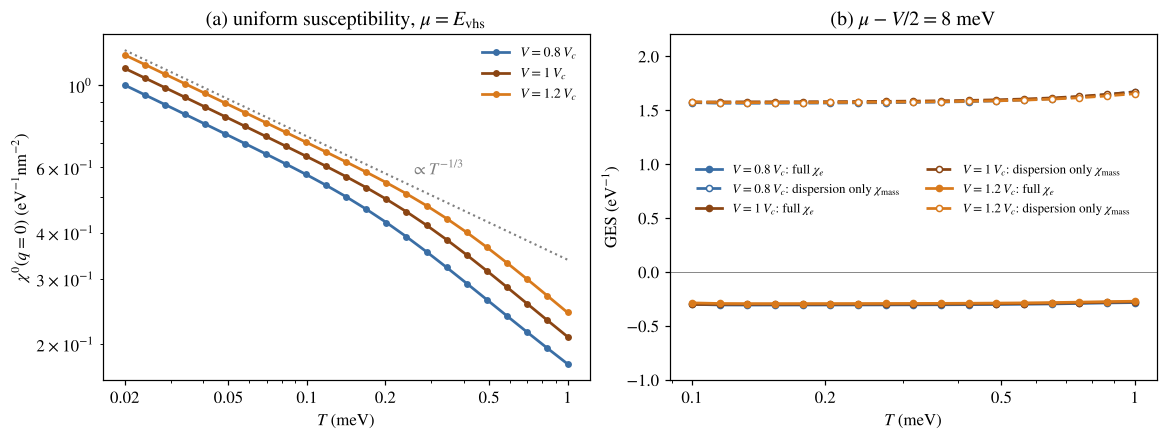
\includegraphics[width=0.85\textwidth]{uniform_susceptibility_ipynb.png}
\caption{(a) Uniform susceptibility at the van Hove energy; dotted line $\propto T^{-1/3}$. (b) GES at $\mu-V/2=8\meV$. Solid: full $\chie$. Dashed: dispersion only, $\chim$. The three biases nearly coincide.}
\label{fig:chi0}
\end{figure}

%======================================================================
\section{Benchmark: the gapped singular saddle point}\label{app:benchmark}
%======================================================================

As a check of the method, and as a point of comparison, we reproduce the setting of Kitamura \emph{et al.}: a two-band model
\begin{equation}
H(\mathbf p)=\frac{p^2}{2M}\sigma_0+\frac{p_xp_y}{M_{xy}}\sigma_x+\Delta\sigma_y+\frac{p_x^2-p_y^2}{2M_{xx}}\sigma_z ,
\end{equation}
with $1/M=1$, $1/M_{xx}=0.5$ and $1/M_{xy}=1.5$. At $\Delta=0$ the lower band has a singular saddle at a quadratic band touching, where the metric diverges as $1/p^2$. A finite $\Delta$ opens a gap $2\Delta$, regularises the metric, and splits the singularity into four ordinary saddles at energy $E_s=-\Delta\sqrt{1-M_{xy}^2/M^2}$ (Fig.~\ref{fig:bench}a). With $\mu=E_s$ and a momentum cutoff $|\mathbf p|\le1$, the mass term is positive, while $\chig$ is negative and grows rapidly as the gap closes (Fig.~\ref{fig:bench}b). For $\Delta=0.17$ the two nearly cancel, and $\chie<0$ only above $T\approx0.01$. For $\Delta=0.02$, $\chie$ is clearly negative at all temperatures shown: the ferromagnetic tendency is geometry driven, as found by Kitamura \emph{et al.} At the monkey saddle the metric stays finite, and this is why geometry decides the sign there only where the dispersion is nearly neutral.

\begin{figure}[h]
\centering
\begin{minipage}[t]{0.40\textwidth}\centering
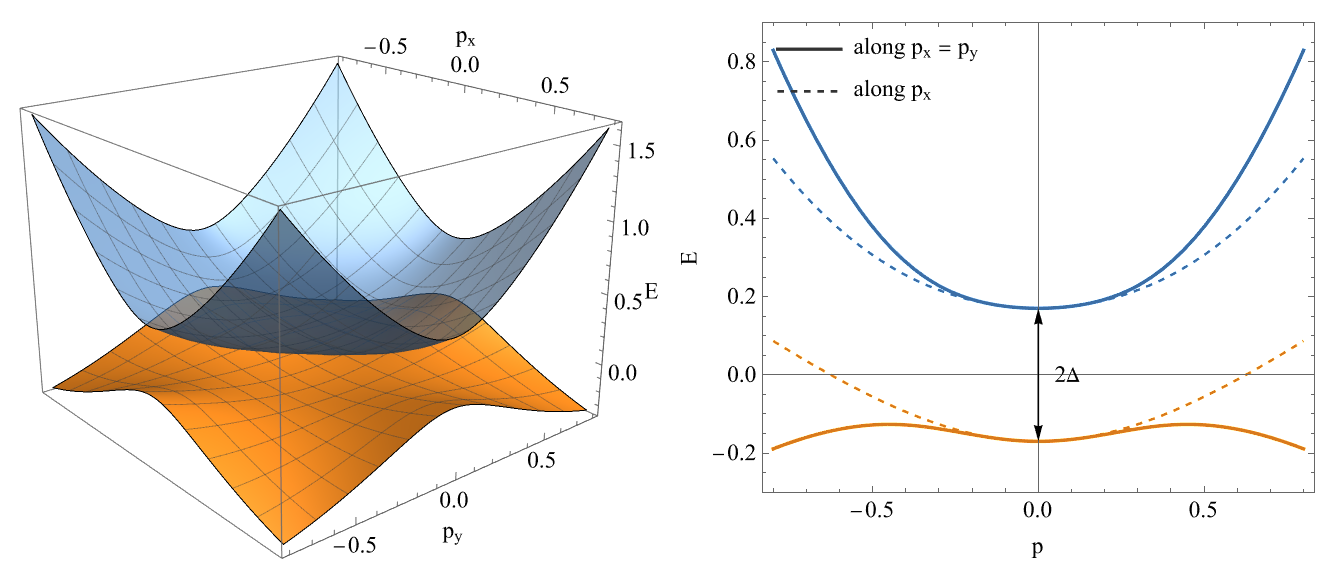
\includegraphics[width=\textwidth]{Gapped_Singular_Saddle.png}\\
{\small (a)}
\end{minipage}\hfill
\begin{minipage}[t]{0.40\textwidth}\centering
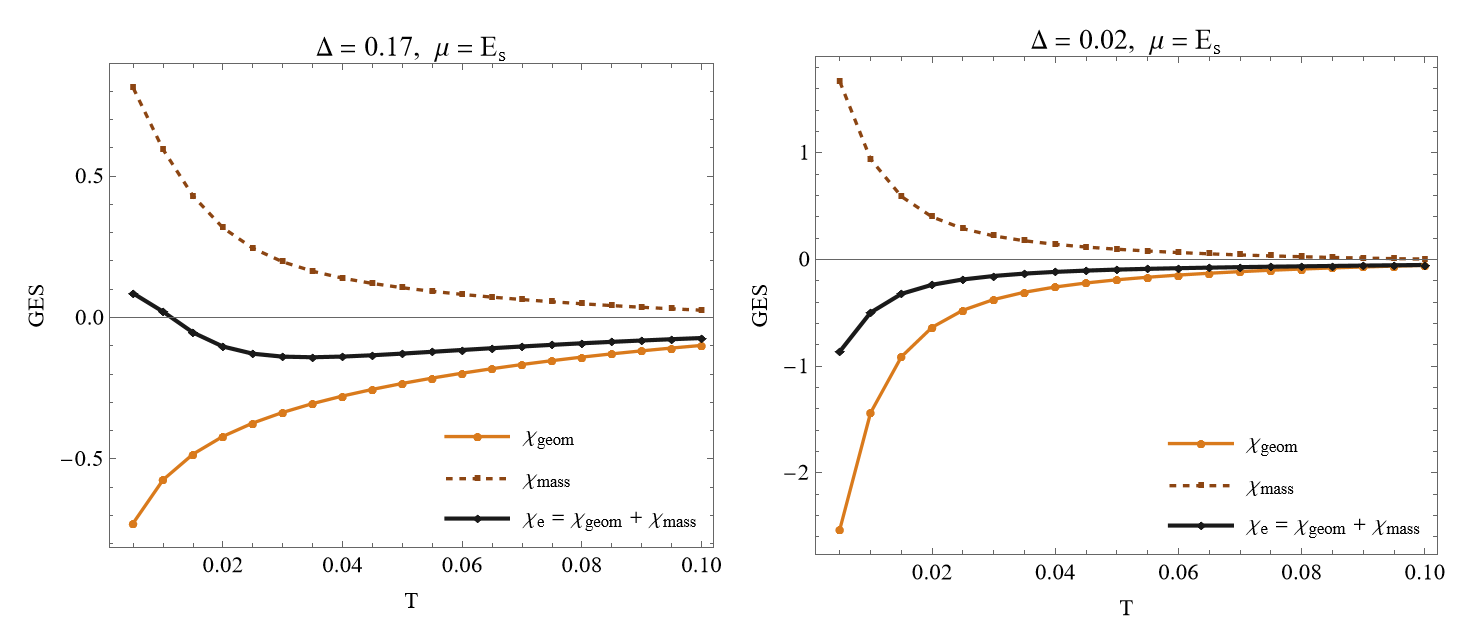
\includegraphics[width=\textwidth]{GES_Singular.png}\\
{\small (b)}
\end{minipage}
\caption{Gapped singular saddle point. (a) Bands for $\Delta=0.17$ (gap $2\Delta$, model units). (b) GES against temperature at the saddle energy for $\Delta=0.17$ and $\Delta=0.02$: $\chig$, $\chim$ and $\chie=\chig+\chim$.}
\label{fig:bench}
\end{figure}

\end{document}
